\documentclass[a4paper, 11pt]{article}
\usepackage[left=2cm, right=2cm,top=2cm,bottom=2cm]{geometry}
\usepackage{graphicx}
\usepackage{graphics}
\usepackage{float}
\usepackage[table,xcdraw]{xcolor}
\usepackage{diagbox}
\usepackage{caption}
\captionsetup{font=small, labelfont=bf, labelformat=empty}
\newlength{\drop}

\begin{document}

% Title Page
\begin{titlepage}
    \drop=0.1\textheight
    \centering
    \vspace*{\baselineskip}
    \rule{\textwidth}{1.6pt}\vspace*{-\baselineskip}\vspace*{2pt}
    \rule{\textwidth}{0.4pt}\\[\baselineskip]
    {\LARGE Parallel Computing - Challenge 1}\\[0.2\baselineskip]
    \rule{\textwidth}{0.4pt}\vspace*{-\baselineskip}\vspace{3.2pt}
    \rule{\textwidth}{1.6pt}\\[\baselineskip]
    \scshape
    Parallel implementation of merge sort using OpenMP \\
    \vspace*{2\baselineskip}
    {\Large Andrea Barletta}
    \vfill
    {\scshape A.Y. 2024/2025}
  \end{titlepage}
\newpage         % Starts a new page

% Sections
\section{Introduction}
The goal of the challenge is to parallelize an existing program that performs the merge sort of a vector.\\
Recalling that the merge sort works as follow:
\begin{enumerate}
    \item Divide array into halves
    \item Call sort on both
    \item Merge
\end{enumerate}
It's clear that this algorithm can benefit from parallelization, particularly in the second step. 
It will also be interesting to compare the performance (measured in execution time) of the serial version against the parallelized version, and to examine the effects of different design choices.
\section{Experimental setup}
The programs were executed on an Apple M1 chip, which features 8 CPU cores. This number is relevant for the way OpenMP creates threads using the "$\#pragma\ omp\ parallel$" directive
\section{Performance measurements}
Each version was run 10 times, and the average execution time was calculated, excluding the minimum and maximum values.\\
The table below shows the execution times (in seconds), where in the parallel version, we create 8 threads and a total of 7 tasks.
\begin{table}[H]
    \centering
    \begin{tabular}{|l|l|l|}
    \hline
    Vector length & Serial time (s) & Parallel time (s) \\ \hline
    80000         & 0.009           & 0.003             \\ \hline
    160000        & 0.012           & 0.005             \\ \hline
    320000        & 0.020           & 0.008             \\ \hline
    640000        & 0.042           & 0.017             \\ \hline
    1280000       & 0.088           & 0.037             \\ \hline
    2560000       & 0.187           & 0.073             \\ \hline
    5120000       & 0.389           & 0.158             \\ \hline
    10240000      & 0.828           & 0.316             \\ \hline
    20480000      & 1.734           & 0.641             \\ \hline
    40960000      & 3.545           & 1.312             \\ \hline
    81920000      & 7.385           & 2.718             \\ \hline
    163840000     & 16.536          & 5.631             \\ \hline
    \end{tabular}
    \end{table}
    \pagebreak
It's also interesting to have a look at a plot of these values, and comparing their growth.
\begin{figure}[H]
    \centering
    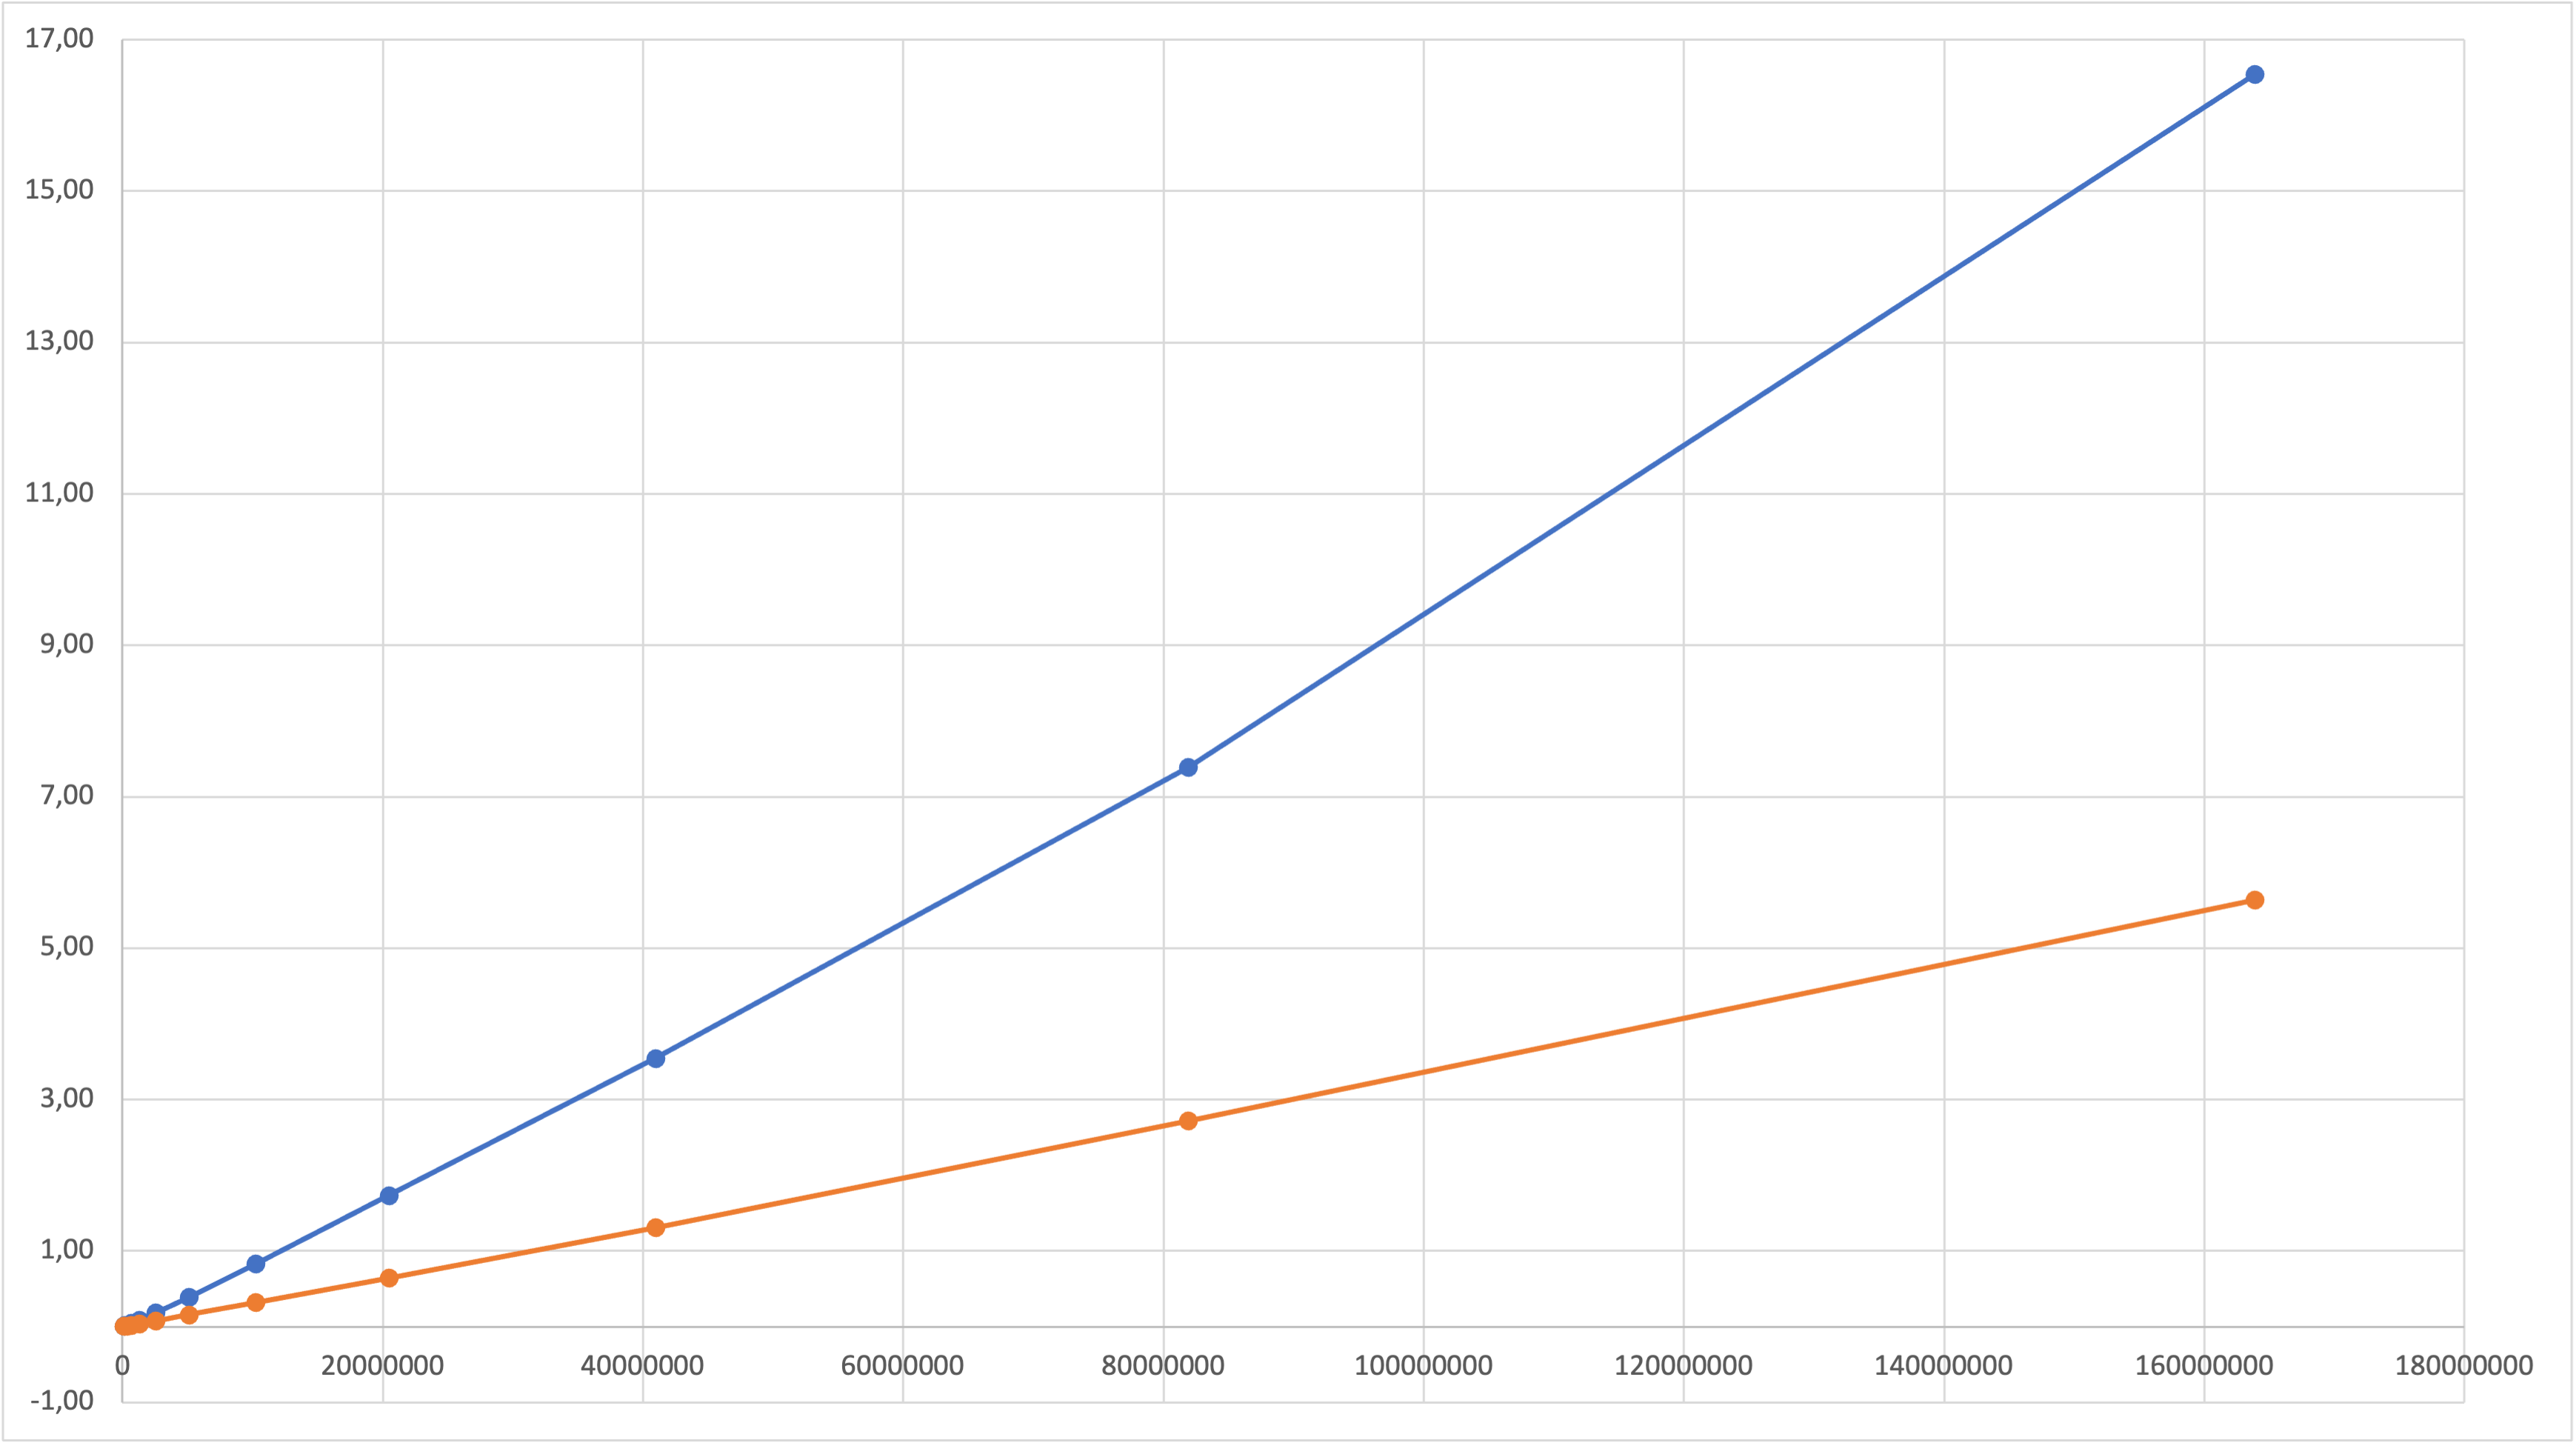
\includegraphics[width=0.7\textwidth]{svp}
    \caption{Blue line: serial version\qquad Orange line: parallel version}
\end{figure}
The parallel version is approximately 3 times faster than the serial version.
\section{Design choices}
Each half of every layer of the merge sort is assigned to a new thread using the task directive.\\
Creating more tasks than threads can lead to a performance slowdown due to the overhead of handling task dispatch. Therefore, after reaching a certain depth in the merge sort tree, the algorithm proceeds sequentially.\\
It's also interesting to explore different configurations, particularly the impact of varying the number of threads and tasks.
\begin{table}[H]
    \centering
    \resizebox{0.7\columnwidth}{!}{
    \begin{tabular}{|c|c|c|c|c|c|c|c|}
    \hline
    \diagbox{\# threads}{\# tasks} & 1                             & 3                             & 7                             & 15                            & 31                            & 63                            & 127                           \\ \hline
    1         & \cellcolor[HTML]{70AD47}4.389 & \cellcolor[HTML]{FFC000}4.429 & \cellcolor[HTML]{FFC000}4.415 & \cellcolor[HTML]{FFC000}4.406 & \cellcolor[HTML]{FFC000}4.681 & \cellcolor[HTML]{FFC000}4.416 & \cellcolor[HTML]{FFC000}4.44  \\ \hline
    2         & \cellcolor[HTML]{70AD47}4.388 & \cellcolor[HTML]{70AD47}2.388 & \cellcolor[HTML]{FFC000}2.361 & \cellcolor[HTML]{FFC000}2.509 & \cellcolor[HTML]{FFC000}2.349 & \cellcolor[HTML]{FFC000}2.356 & \cellcolor[HTML]{FFC000}2.365 \\ \hline
    4         & \cellcolor[HTML]{70AD47}4.4   & \cellcolor[HTML]{70AD47}2.352 & \cellcolor[HTML]{FFC000}1.321 & \cellcolor[HTML]{FFC000}1.848 & \cellcolor[HTML]{FFC000}1.622 & \cellcolor[HTML]{FFC000}1.616 & \cellcolor[HTML]{FFC000}1.621 \\ \hline
    8         & \cellcolor[HTML]{70AD47}4.467 & \cellcolor[HTML]{70AD47}2.333 & \cellcolor[HTML]{70AD47}1.333  & \cellcolor[HTML]{68349A}1.023 & \cellcolor[HTML]{FFC000}1.175 & \cellcolor[HTML]{FFC000}1.196 & \cellcolor[HTML]{FFC000}1.168 \\ \hline
    \rowcolor[HTML]{FF0000} 
    16        & 4.41                          & 2.48                          & 1.347                         & 1.064                         & 0.976                         & 1.033                         & 1.021                         \\ \hline
    \rowcolor[HTML]{FF0000} 
    32        & 4.406                         & 2.341                         & 1.322                         & 1                             & 1.012                         & 1.1                           & 0.983                         \\ \hline
    \rowcolor[HTML]{FF0000} 
    64        & 4.409                         & 2.347                         & 1.368                         & 1.13                          & 1.03                          & 0.988                         & 1.037                         \\ \hline
    \end{tabular}
    }
\end{table}
The red area indicates a configuration where there are more threads than CPU cores, resulting in little to no improvement. The orange area shows configurations where there are more tasks than threads, with minimal improvement despite increased resource usage.\\
The most efficient configuration, in terms of threads and tasks used relative to performance, is 8 threads and 15 tasks (purple value).\\
It's slightly faster than our initial approach since we can benefit from an extra task assigned to the remaining thread.\\
The execution times for all the test vector lengths are reported in the table below
\begin{table}[H]
    \centering
    \resizebox{\columnwidth}{!}{
        \begin{tabular}{|l|l|l|l|l|l|l|l|l|l|l|l|l|}
        \hline
        \multicolumn{1}{|c|}{\# elements} & 80000 & 160000 & 320000 & 640000 & 1280000 & 2560000 & 5120000 & 10240000 & 20480000 & 40960000 & 81920000 & 163840000 \\ \hline
        time (s)                          & 0.001 & 0.004  & 0.007  & 0.015  & 0.028   & 0.6     & 0.127   & 0.231    & 0.494    & 0.976    & 2.09     & 4.136     \\ \hline
        \end{tabular}
    }
\end{table}
\end{document}
